%
% wurzel2.tex
%
% (c) 2021 Prof Dr Andreas Müller, OST Ostschweizer Fachhochschule
%
\begin{frame}[t]
\setlength{\abovedisplayskip}{5pt}
\setlength{\belowdisplayskip}{5pt}
\frametitle{$\mathbb{Z}(\sqrt{2})\only<7->{ = \mathbb{Z}[X]/(X^2-2)}$}
\vspace{-20pt}
\begin{columns}[t,onlytextwidth]
\begin{column}{0.48\textwidth}
\begin{block}{Der Ring $\mathbb{Z}(\sqrt{2})$}
$\mathbb{Z}(\sqrt{2})$ als Teilring:
{\color{blue}
\[
R=\{ a+b\sqrt{2}\;|\; a,b\in\mathbb{Z} \} \subset \mathbb{R}
\]}%
\uncover<2->{$\sqrt{2}\not\in\mathbb{Q}$}\uncover<3->{
$\Rightarrow$
$1$ und $\sqrt{2}$ sind inkommensurabel}\uncover<4->{
$\Rightarrow$
$R$ dicht in $\mathbb{R}$}
\end{block}
\uncover<5->{%
\begin{block}{Algebraische Konstruktion}
\uncover<8->{%
Das Polynom $X^2-2$ ist irreduzibel als Polynom in $\mathbb{Q}[X]$}
\[
\uncover<8->{\mathbb{Z}[X]/(X^2-2)
=}
{\color{red}\{a+bX\;|\;a,b\in\mathbb{Z}\}}
\]\uncover<7->{%
mit Rechenregel: $X^2=2$}
\end{block}}
\uncover<9->{%
\begin{block}{Körper}
$\mathbb{Q}(\sqrt{2}) = \mathbb{Q}[X]/(X^2-2)$
\end{block}}
\end{column}
\begin{column}{0.48\textwidth}
\begin{center}
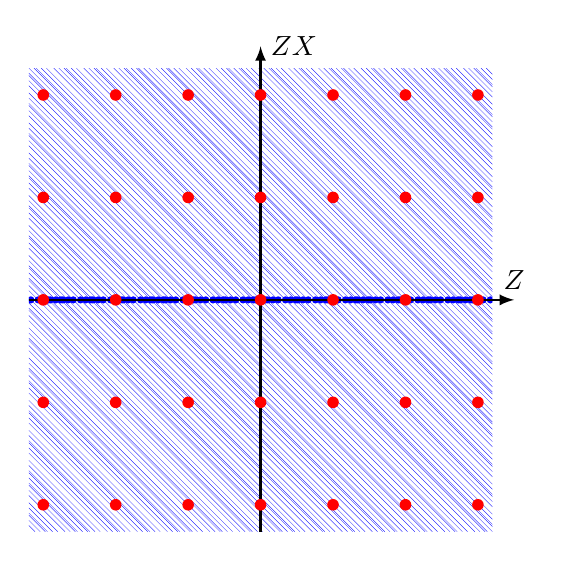
\begin{tikzpicture}[>=latex,thick,scale=0.92]
\begin{scope}
\clip (-3.2,-3.2) rectangle (3.2,3.2);
\foreach \x in {-10,...,10}{
	\pgfmathparse{int(\x/sqrt(2))-5}
	\xdef\s{\pgfmathresult}
	\pgfmathparse{int(\x/sqrt(2))+5}
	\xdef\t{\pgfmathresult}
	\foreach \y in {\s,...,\t}{
		\uncover<4->{
			\fill[color=blue] ({\x-\y*sqrt(2)},0)
				circle[radius=0.05];
		}
		\uncover<6->{
			\draw[color=blue,line width=0.1pt] 
				({\x-\y*sqrt(2)-3.2},3.2) 
				--
				({\x-\y*sqrt(2)+3.2},-3.2);
		}
	}
}
\end{scope}

\draw[->] (-3.2,0) -- (3.5,0) coordinate[label={$\mathbb{Z}$}];

\uncover<5->{
	\draw[->] (0,-3.2) -- (0,3.5) coordinate[label={right:$\mathbb{Z}X$}];

	\foreach \x in {-3,...,3}{
		\foreach \y in {-2,...,2}{
			\fill[color=red]
				({\x},{\y*sqrt(2)}) circle[radius=0.08];
		}
	}
}

\end{tikzpicture}
\end{center}
\end{column}
\end{columns}
\end{frame}
